\documentclass{article}
 
\author{Sam Ionesi \and Nathaniel Van \and John Bush}
\title{Lab 1} 

\usepackage{fancyvrb}
\usepackage{amsmath}
\usepackage{multirow} 
\usepackage{eqparbox}
\usepackage{booktabs} 
\usepackage{graphicx} 
\usepackage{placeins} 
\usepackage{siunitx} 
\usepackage{listings} 
\usepackage{commath}

\numberwithin{figure}{section} 
\numberwithin{table}{section} 

\begin{document} 

\maketitle

\section{Introduction} 

\subsection{Question} 

To what extent does the given spring behave as an ideal spring?

\subsection{Hypothesis} 

As seen previously in physics class, the force exerted by an ideal spring is modeled by Hooke's Law, $F = -kx$, where $k$ is the spring-force constant. This $k$ is considered, in the ideal spring, to be a fixed scalar value and a property intrinsic to the spring.  While this model is precise for most practical purposes, a real, non-ideal spring will not conform to this model.

In order to recognize how regularly the spring conforms to the model of the ideal spring, we observe and compare how the spring oscillates over a range of forces and displacements.  By suspending weights of varying mass from the spring and displacing those weights, we create an oscillation that can be measured and allow the spring force constant to be calculated.  In an ideal spring, the spring-force constant would be constant.  Observing a variation in this value would indicate conditions where the spring deviates from the ideal modeled by Hooke's Law.

\subsection{Method} 

\begin{figure}[!hbp]
    \begin{tabular}{rl} 
        \toprule
        Equipment & Purpose \\
        \midrule
        Ring stand & Suspend the spring and mass. \\
        Spring & Spring whose characteristics are observed. \\
        Hanging masses & Masses range from 10 g to 1 kg. \\
        Meter stick & To estimate displacement from equilibrium. \\
        Motion detector & Record displacement of spring at regular intervals of time. \\
        Labquest & Control the motion detector and receive data. \\
        Computer & Control the Labquest controller and receive data. \\
        1 Note Card & Act as reflector for motion detector. \\
        Tape & Fix the note card to the suspended mass. \\ 
        \bottomrule
    \end{tabular} 
    \caption{Equipment used in experiment.} 
\end{figure} 


\begin{figure}[!hbp]
    \centering
    \includegraphics[width=\textwidth]{setup.jpg}
    \caption{Experiment setup}
\end{figure} 



\begin{enumerate} 
	\item Setup the rig displayed in the diagram below.
	\item Place tape on the bottom of the mass to hold the note card.
	\item Pull the mass down directly above the motion detector from the spring’s equilibrium 2 inches down and release.
	\item Record data using the Labquest.
	\item Find the period of each mass.
	\item Test various weights to see how that affects the “k” value.
	\item Repeat steps as needed. 
\end{enumerate} 



\subsection{Predictions} 

We expect that the frequency of the spring oscillation should be consistent and regular until we add very large masses.  With larger masses, at the extremes of force and displacement, the spring will deform and no longer behave as an ideal spring.

\section{Analysis} 

\subsection{Method} 

Per Hooke's Law, the position can be represented as a function of time as a solution to the differential equation, 
\begin{equation} 
	m \od[2]{x}{t} = -kx 
\end{equation} 
where $x$ is the position of the spring, $t$ is time, $m$ is the mass on the spring, and $k$ is the spring force constant.  It can be seen that $x = A \cos \left( \omega t \right)$ is a solution to this equation, where $\omega^2 = \frac{k}{m}$.  This implies that the frequency of the spring oscillations is a function of the mass and spring force constant, and can easily be obtained by modeling the spring's motion as a sinusoidal function.

It would be difficult to calculate frequency of the spring oscillations directly, as the sampling rate of the motion detector was relatively low, but could be interpolated using the model.  The data was fit to a cosine function by least-squares fitting with a Python script.

The data for each trial, as exported by the Labview software, was fir to a cosine function using the SciPy.optimize package's leastsq method.  This implements the Levenberg-Marquardt algorithm.  The initial paramters were estimated by reviewing the data.  Iterating over the data points, the local peaks were idtentified (as local maxima above the mean) and frequency was estimated to be the mean of the distances between them.  Amplitude was estimated to be half the distance between minimum and maximum position values.  Phase off-set was guessed from the time of the first local maximum in position, and the position off-set was taken from the mean of all position values.  For some trials, the bottom of the mass was within the minimum range of the motion detector and yielded a position value near that boundary of range.  It was thus necessary to filter out position values in that region.

The curve-fitting algorithm calculated the modeling function's frequency term, $\omega$.  As stated above, Hooke's Law would imply that the spring force constant $k$ can be expressed $k = m \omega^2$.  Thus, the spring force constant could quickly be calculated from the results of the curve fitting algorithm.

\clearpage
\subsection{Observed Results} 

\FloatBarrier

\begin{figure}[!hbp]
    \centering
    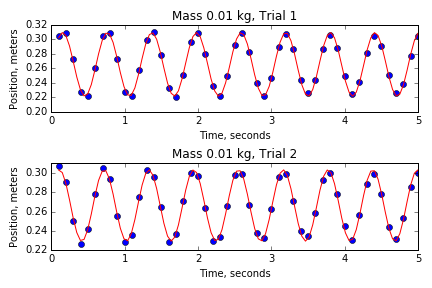
\includegraphics[width=\textwidth]{{data/mass0.01kg}.png}
    \caption{Mass 0.01 kg, Position-Time}
\end{figure}


\begin{figure}[!hbp]
    \centering
    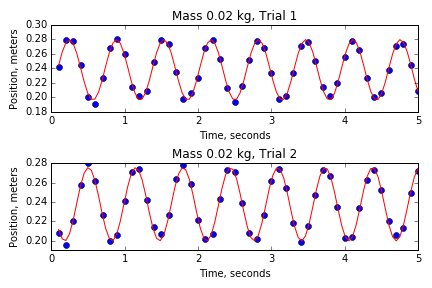
\includegraphics[width=\textwidth]{{data/mass0.02kg}.png}
    \caption{Mass 0.02 kg, Position-Time}
\end{figure}


\begin{figure}[!hbp]
    \centering
    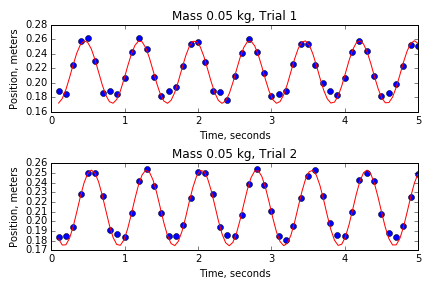
\includegraphics[width=\textwidth]{{data/mass0.05kg}.png}
    \caption{Mass 0.05 kg, Position-Time}
\end{figure}


\begin{figure}[!hbp]
    \centering
    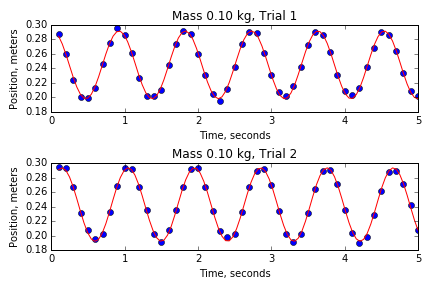
\includegraphics[width=\textwidth]{{data/mass0.10kg}.png}
    \caption{Mass 0.10 kg, Position-Time}
\end{figure}


\begin{figure}[!hbp]
    \centering
    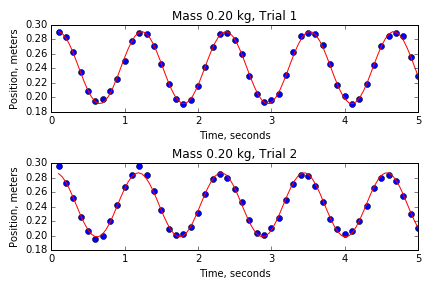
\includegraphics[width=\textwidth]{{data/mass0.20kg}.png}
    \caption{Mass 0.20 kg, Position-Time}
\end{figure}


\begin{figure}[!hbp]
    \centering
    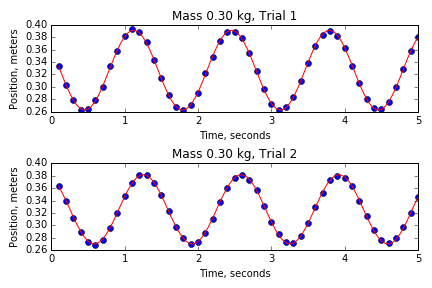
\includegraphics[width=\textwidth]{{data/mass0.30kg}.png}
    \caption{Mass 0.30 kg, Position-Time}
\end{figure}


\begin{figure}[!hbp]
    \centering
    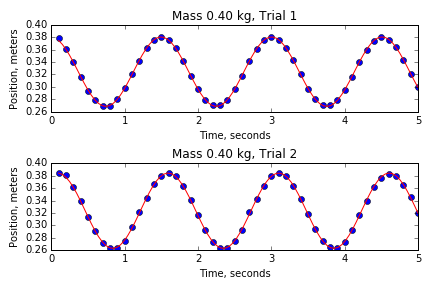
\includegraphics[width=\textwidth]{{data/mass0.40kg}.png}
    \caption{Mass 0.40 kg, Position-Time}
\end{figure}


\begin{figure}[!hbp]
    \centering
    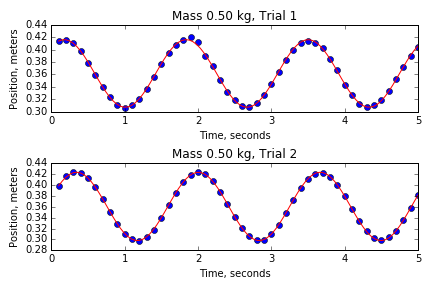
\includegraphics[width=\textwidth]{{data/mass0.50kg}.png}
    \caption{Mass 0.50 kg, Position-Time}
\end{figure}


\begin{figure}[!hbp]
    \centering
    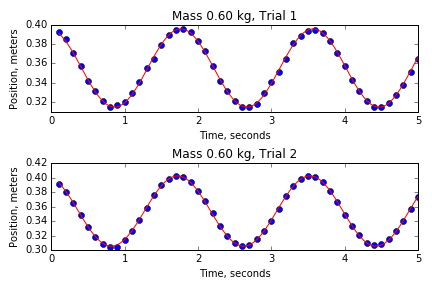
\includegraphics[width=\textwidth]{{data/mass0.60kg}.png}
    \caption{Mass 0.60 kg, Position-Time}
\end{figure}


\begin{figure}[!hbp]
    \centering
    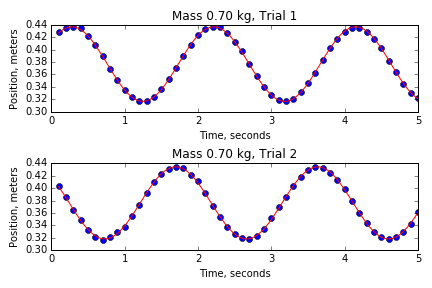
\includegraphics[width=\textwidth]{{data/mass0.70kg}.png}
    \caption{Mass 0.70 kg, Position-Time}
\end{figure}


\begin{figure}[!hbp]
    \centering
    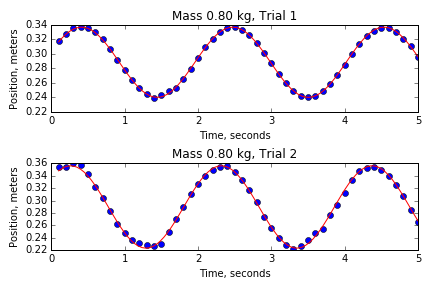
\includegraphics[width=\textwidth]{{data/mass0.80kg}.png}
    \caption{Mass 0.80 kg, Position-Time}
\end{figure}


\begin{figure}[!hbp]
    \centering
    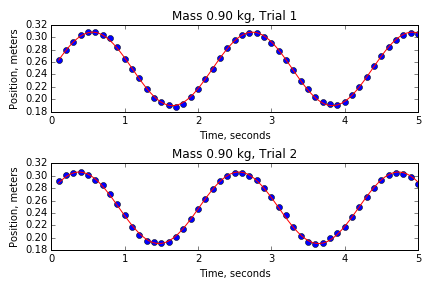
\includegraphics[width=\textwidth]{{data/mass0.90kg}.png}
    \caption{Mass 0.90 kg, Position-Time}
\end{figure}


\begin{figure}[!hbp]
    \centering
    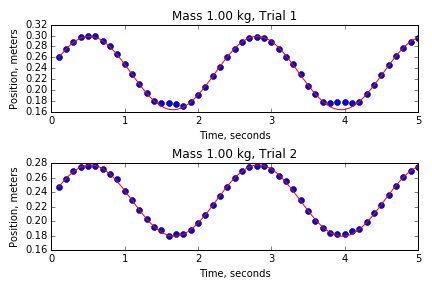
\includegraphics[width=\textwidth]{{data/mass1.00kg}.png}
    \caption{Mass 1.00 kg, Position-Time}
\end{figure}


\begin{figure}[!hbp]
    \centering
    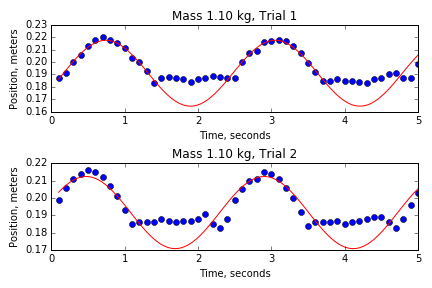
\includegraphics[width=\textwidth]{{data/mass1.10kg}.png}
    \caption{Mass 1.10 kg, Position-Time}
\end{figure}

\FloatBarrier

\begin{tabular}{lll} 
        \toprule
		Mass (kg) & Angular Frequency & Spring Constant \\
                    & ($\omega$) & ($k$) \\ 
        \midrule 
		0.01 & 10.3310 & 1.0673 \\ 
		& 10.295266 & 1.059925 \\
		0.02 & 9.7465 & 1.8999 \\ 
		& 9.730597 & 1.893690 \\
		0.05 & 8.3888 & 3.5186 \\ 
		& 8.367833 & 3.501032 \\
		0.10 & 6.9505 & 4.8309 \\ 
		& 6.953125 & 4.834595 \\
		0.20 & 5.4843 & 6.0154 \\ 
		& 5.562774 & 6.188890 \\
		0.30 & 4.7049 & 6.6407 \\ 
		& 4.709160 & 6.652855 \\
		0.40 & 4.1710 & 6.9590 \\ 
		& 4.167170 & 6.946121 \\
		0.50 & 3.7790 & 7.1403 \\ 
		& 3.783115 & 7.155981 \\
		0.60 & 3.4844 & 7.2847 \\ 
		& 3.482183 & 7.275358 \\
		0.70 & 3.2472 & 7.3812 \\ 
		& 3.246760 & 7.379013 \\
		0.80 & 3.0472 & 7.4283 \\ 
		& 3.057934 & 7.480769 \\
		0.90 & 2.8813 & 7.4715 \\ 
		& 2.885437 & 7.493171 \\
		1.00 & 2.7425 & 7.5215 \\ 
		& 2.741550 & 7.516096 \\
		1.10 & 2.7199 & 8.1374 \\ 
		& 2.588541 & 7.370601 \\ 
        \bottomrule
\end{tabular} 

\begin{figure}[!hbp]
    \centering
    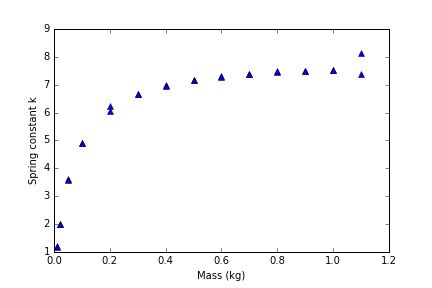
\includegraphics[width=\textwidth]{data/mass-v-k.png}
    \caption{Mass (kg) - Spring Constant k} 
    \label{mkplot}
\end{figure} 

\FloatBarrier 

\subsection{Interpretation} 

As can be observed in Figure~\ref{mkplot}, the calculated spring force constant is relatively consistent for masses between 200 g and 1 kg.  At smaller masses, the calculated spring force constant deviates considerably from the other values and appears to increase at a logarithmic rate.  There is also variance with masses above 1 kg, but as it was difficult to accurately record the displacement with those masses, this may reflect the limitations of the experimental setup.

The spring proved to be very stiff and resilient.  It is possible that with small masses, the suspended mass was bouncing or swinging at the point where it was fastended to the spring.  This would skew calculations considerably, as it would essentially become a two-oscillator (a pendulum as well as a spring) system.  It could also be that the physical characteristics of the spring, the flexing and stiffness of the metal, varies at very small displacements.  In any case, the ideal spring model was not consistent with very small masses.

The spring was expected to break down with the greatest masses, but it was much more resislient than expected and was relatively consistent at the largest displacements we were able to observe.  The spring behaves very near the ideal model for the greatest displacements that were pracitically achieved in the laboratory conditions.

There did appear to be some observable inconsistency in the spring force constant with masses in the range of 200 g and 1 kg.  With additional data points it may be possible to perform a statistical regression and develop a more precise model of the spring force constant as it varies with displacement.

\end{document} 